\documentclass[a4paper, 12pt]{article}%тип документа

%отступы
\usepackage[left=2cm,right=2cm,top=2cm,bottom=3cm,bindingoffset=0cm]{geometry}

%Русский язык
\usepackage[T2A]{fontenc} %кодировка
\usepackage[utf8]{inputenc} %кодировка исходного кода
\usepackage[english,russian]{babel} %локализация и переносы

%Вставка картинок
\usepackage{wrapfig}
\usepackage{graphicx}
\graphicspath{{pictures/}}
\DeclareGraphicsExtensions{.pdf,.png,.jpg}

%оглавление
\usepackage{titlesec}
\titlespacing{\chapter}{0pt}{-30pt}{12pt}
\titlespacing{\section}{\parindent}{5mm}{5mm}
\titlespacing{\subsection}{\parindent}{5mm}{5mm}
\usepackage{setspace}

%Графики
\usepackage{multirow}
\usepackage{pgfplots}
\pgfplotsset{compat=1.9}

%Математика
\usepackage{amsmath, amsfonts, amssymb, amsthm, mathtools}

%Стиль страницы
\usepackage{fancyhdr}
\pagestyle{fancy}

\begin{document}

\begin{titlepage}

\begin{center}
%\vspace*{1cm}
\large\textbf{Московский Физико-Технический Институт}\\
\large\textbf{(национальный исследовательский университет)}
\vfill
\line(1,0){430}\\[3mm]
\huge\textbf{Лабораторная работа №4.7.1}\\
\large\textbf{Двойное лучепреломление}\\
\line(1,0){430}\\[1mm]
\vfill
\large Баканова К.В., Б01-003\\
%\vspace*{1cm}
\large март 2022 г.\\
\end{center}

\end{titlepage}
\section*{Теория}
\subsection*{Плоские волны в кристаллах}
\begin{equation}
\text{rot} \vec{H} = \dfrac{1}{c}\dfrac{\partial \vec{D}}{\partial t}, \text{rot} \vec{E} = -\dfrac{1}{c}\dfrac{\partial \vec{B}}{\partial t}
\end{equation}
Если среды прозрачны и однородны то в них распорстраняются волны:
\begin{equation}
\vec E = \vec{E}_0 e^{i(\omega t - \vec{k}\vec{r})}, \vec{H} = \vec{H}_0e^{i(\omega t - \vec{k}\vec{r})}
\end{equation}
Введем единичный вектор нормали к скорости распространения волны $\vec{N}$ и направим его вдоль скорости, тогда
\begin{equation}
\vec{D} = -\dfrac{c}{v}\left[\vec{N}, \vec{H}\right], \vec{B} = \dfrac{c}{v}\left[	\vec{N}, \vec{E}\right]
\end{equation}
\subsection*{Оптические одноосные кристаллы}
Введем \textit{тензор диэлектрической проницаемости} $\varepsilon$ ($\vec{D} = \varepsilon \vec{E}$). Все его значения описываются эллипсоидом инерции. 

В кристаллах этот эллипсоид --- эллипсоид вращения. В них оптическая ось --- ось вращения эллипсоида. В них принято обозначать $\varepsilon_{\parallel} = \varepsilon_z, \varepsilon_{\perp} = \varepsilon_x = \varepsilon_y$

\begin{equation}
\vec{D}_{\parallel} = \varepsilon_{\parallel} \vec{E}_{\parallel},\vec{D}_{\perp} = \varepsilon_{\perp} \vec{E}_{\perp} 
\end{equation}

Можно показать, что угол $\theta$ между волновой нормалью и осью вращения эллипсоида при разделении $\vec{D}$ на $\vec{D}_e$ --- лежащая в главном сечении и $\vec{D}_o$ --- нормальная составляющая такой, что
\begin{equation}
\sin \theta = \dfrac{D_{e\parallel}}{D_e}, \cos \theta = \dfrac{D_{e\perp}}{D_e}
\end{equation}
\begin{equation}
n = \dfrac{1}{\sin A}\sqrt{\sin^2 \phi_1 + \sin^2 \phi_2 + 2 \sin \phi_1 \sin \phi_2 \cos A}
\end{equation}
Из этого, если $n_o - n_e \ll n_o$ и $n_e$, то 
\begin{equation}
n(\theta) \approx n_e + (n_o - n_e) \cos^2 \theta
\end{equation}
%\newpage
\subsection*{Двойное лучепреломление в призме исландского шпата}
\begin{wrapfigure}{r}{0.3\textwidth}
  \begin{center}
    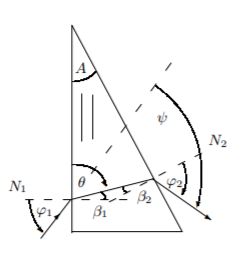
\includegraphics[width = 0.2\textwidth]{1.png}
  \end{center}
  \caption{Ход луча в призме}
\end{wrapfigure}
При таком ходе луча и расположении призмы у нас повторяется ситуация из предыдущего параграфа теории. Тогда, можно посчитать показатель преломления изотропной среды по формуле 
\begin{equation}
n = \dfrac{\sin\left(\dfrac{\psi_m + A}{2}\right)}{\sin \left(\dfrac{A}{2}\right)}
\end{equation}
Здесь $\psi_m$  --- минимальный угол, на который призма преломляет луч.
Если призма неизотропна, то этой формулой, строго говоря, можно воспользоваться только для обыкновенной волны, которая, как это было показано ранее, распространяется так же, как и в изотропной среде. 
\section*{Экспериментальная установка}

\begin{figure}[h]
\begin{center}
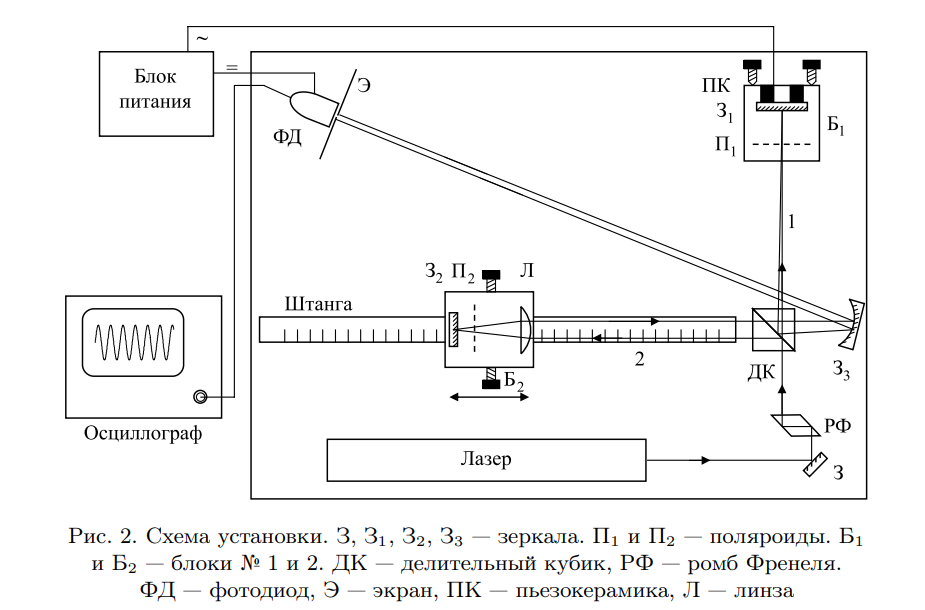
\includegraphics[width = 0.7\textwidth]{2.png}
\caption{Экспериментальная установка}
\end{center}
\end{figure}
\begin{equation}
\phi_2 = A + \psi - \phi_1
\end{equation}
Длина волны источника (Na-Ne): $\lambda_{Na-Ne} = 0,63$ мкм.
\section*{Ход работы}
\begin{enumerate}
\item Отъюстируем систему, то есть сделаем так, что луч проходит через 0 и 180.
\item Определим угол А, для этого добьемся, чтобы отраженный луч шел ровно назад для меньшего катета ($\theta_1$) и гипотенузы ($\theta_2$). По формуле 
\[A = 180^{\circ} - (\theta_1 - \theta_2)\]
Найдем A
\[\theta_1 = (297 \pm 2)^{\circ}\]
\[\theta_2 = (154 \pm 2)^{\circ}\]
\[A = (37 \pm 2)^{\circ}\]
\item Определим разрешенное направление поляризатора. Для этого направив его на видимый свет, установим его в положение наименьшего пропускания.
\item Получаем изображение на лимбе как на рис. 5.
\item Вращая столик, снимем зависимость углов отклонения волн от угла падения, запишем данные в таблицу 1.
\item Далее с помощью программы рассчитаем все данные, необходимые для работы и построим график.
  \begin{center}
    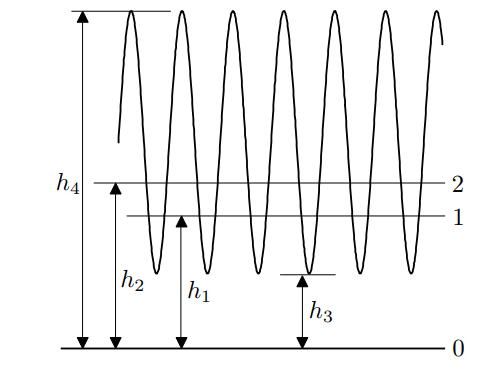
\includegraphics[width = 0.6\textwidth]{3.png}
  \end{center}
\begin{center}
\begin{tabular}{|c|c|c|c|c|c|c|c|c|c|c|c|c|c|}
\hline
$\phi_1, ^{\circ}$             & 10     & 15     & 20     & 30    & 40    & 50     & 60    & 70    \\ \hline
$\delta_{\phi_1}, ^{\circ}$    & 2      & 2      & 2     & 2     & 2     & 2     & 2     & 2     \\ \hline
$\psi_0, ^{\circ}$             & 31     & 30     & 28   & 26     & 27    & 29     & 32    & 37    \\ \hline
$\delta_{\psi_o},  ^{\circ}$   & 2      & 2      & 2     & 2     & 2     & 2     & 2     & 2     \\ \hline
$\psi_e, ^{\circ}$             & 21     & 21     & 20    & 20    & 21    & 23    & 27    & 32    \\ \hline
$\delta_{\psi_e}, ^{\circ}$    & 2      & 2      & 2     & 2     & 2     & 2     & 2     & 2      \\ \hline
$\phi_{2o},  ^{\circ}$         & 58     & 52     & 45    & 33    & 24    & 16    & 9     & 4     \\ \hline
$\delta_{\phi_{2o}}, ^{\circ}$ & 6      & 6      & 6     & 6     & 6     & 6     & 6     & 6     \\ \hline
$\phi_{2e}, ^{\circ}$          & 48     & 43     & 37    & 27     & 18    & 10     & 4     & -1    \\ \hline
$\delta_{\phi_{2e}}, ^{\circ}$ & 6      & 6      & 6     & 6     & 6     & 6     & 6     & 6     \\ \hline
$\theta_o, ^{\circ}$           & 84     & 81     & 78    & 72    & 67    & 63    & 58    & 55    \\ \hline
$\delta_{\theta_o}, ^{\circ}$  & 6      & 5      & 4     & 4     & 4      & 3     & 3     & 3     \\ \hline
$\theta_e, ^{\circ}$           & 83     & 80     & 77    & 71    & 65    & 60    & 56     & 52    \\ \hline
$\delta_{\theta_e}, ^{\circ}$  & 6      & 4      & 4     & 4     & 4     & 3     & 3     & 3     \\ \hline
$\cos^2\theta_o$               & 0,0111 & 0,0239 & 0,042 & 0,092 & 0,150 & 0,212 & 0,274 & 0,322 \\ \hline
$\delta_{\cos^2\theta_o}$      & 0,0007 & 0,0014 & 0,002 & 0,005 & 0,008 & 0,011 & 0,015 & 0,017 \\ \hline
$\cos^2\theta_e$               & 0,0139 & 0,0298 & 0,052 & 0,111 & 0,181 & 0,256 & 0,319 & 0,37  \\ \hline
$\delta_{\cos^2\theta_e}$      & 0,0009 & 0,0016 & 0,003 & 0,006 & 0,010 & 0,014 & 0,017 & 0,02  \\ \hline
$n_o$                          & 1,65   & 1,67   & 1,66  & 1,65  & 1,66  & 1,66  & 1,65  & 1,66  \\ \hline
$\delta_{n_o}$                 & 0,11   & 0,10   & 0,09  & 0,09  & 0,09  & 0,09  & 0,09  & 0,09  \\ \hline
$n_e$                          & 1,48   & 1,50   & 1,49  & 1,50  & 1,51  & 1,51  & 1,53  & 1,54  \\ \hline
$\delta_{n_e}$                 & 0,10   & 0,09   & 0,08  & 0,08  & 0,08  & 0,08  & 0,08  & 0,08  \\ \hline
\end{tabular}
\end{center}
\begin{center}
\caption{Табл. 1: Измеренные и все полученные данные в ходе эксперимента}
\end{center}
\newpage
\item Из графика мы получаем, что главные значения показателей преломления 
\[n_o = 1,66 \pm 0,11\]
\[n_e = 1,49 \pm 0,09\]
\item Теперь из серии измерений мы получаем, что 
\[\psi_{mo} = (26 \pm 1,5) ^ {\circ}\]
\[\psi_{me} = (20 \pm 1,5) ^ {\circ}\]
Отсюда, из формулы $(8)$ получаем, что 
\[n_o = 1,65 \pm 0,09\]
\[n_e = 1,50 \pm 0,09\]
\item Определим углы, соответствующие полному внутреннему отражению
\[\phi_{1o} = (-0,5 \pm 1) ^{\circ}\]
\[\phi_{1e} = (-7,5 \pm 1) ^{\circ}\]
Из этого, принимая, так как полное внтуреннее отражение, $\phi_2 = 90^{\circ}$ из формулы $(6)$ получаем, что 
\[n_o = 1,6 \pm 0,2\]
\[n_e = 1,5 \pm 0,2\]
\end{enumerate}
\section*{Вывод}
В итоге, мы подтвердили, что показатели преломления соответствующих волн соответствуют уже известным. Так же мы установили, что самый точный метод расчета показателей преломления --- по наклону графика $n$ от $\cos^2\theta$.
\end{document}